\documentclass{article}
\usepackage[letterpaper, margin=1in]{geometry}
\usepackage{booktabs}
\usepackage{float}
\usepackage{hyperref}
\usepackage{color}
\usepackage{soul}
\usepackage{tikz}
\usepackage{amssymb}

\hypersetup{
	colorlinks=true,
	linkcolor=black,
	urlcolor=black,
	linktoc=all
}

\title{\Huge Homework 2
	\\\LARGE Artificial Intelligence
	\\\LARGE CS 540 Section 3
	\vspace{2pc}
	}

\author{Ritvik Upadhyaya}
\date{}

\begin{document}

	\maketitle
	\newpage

	\tableofcontents

	\newpage
	\renewcommand\thesubsection{\thesection.\alph{subsection}}
	\section{Genetic Algorithms}
	\subsection{Mating Events}
		\underline{Case 1:}\\
		Mating between chips 4 and 6: 0000110011 \hspace{1pc}\&\hspace{1pc} 0111110010\\
		\\
		\underline{Case 2:}\\
		Mating between chips 1 and 3: 0100010010 \hspace{1pc}\&\hspace{1pc} 1101110011\\
		\\
		\underline{Case 3:}\\
		Mating between chips 5 and 6: 1000001111 \hspace{1pc}\&\hspace{1pc} 0100110001\\
	\subsection{Mutation Events}
		Mutation events are rare occurances of errors during the copying of chromosomes that can result in the following characteristics:
		\begin{itemize}
			\item changes that make the produced chip/organism worse off or "weaker" than the original one.
			\item changes that make the produced chip/organism better off or "stronger" than the original one.
			\item changes that make the produced chip/organism neither better nor worse off than the original one.
		\end{itemize}
		These events are used to get one or more members of a population out of a local minimum or maximum space and discover new potential minimum and maximum spaces that might be better.
	\subsection{GA vs Hillclimbing Algorithm}
		The fact that unlike in traditional hillclimbing algorithms, mutation and crossover move the population away from the local optima in genetic algorithms. This is the reason why genetic algorithms do not stay at the local optima and are also not susceptible to it.
	\section{Simulated Annealing}
	\subsection{Table}
	\vspace{-1pc}
	\begin{table}[H]
		\centering

		\caption{Question 2}

		\label{tab:table1}

		\begin{tabular}{|c|c|c|c|c|c|c|}

			\toprule
			\# of Iterations & $\Delta$E & $\Delta$E$>$0 & \multicolumn{1}{|p{2cm}|}{\centering Temperature \\ (T)} & \multicolumn{1}{|p{2cm}|}{\centering $e^{E/T}$\\(Random \#)} & \multicolumn{1}{|p{1.75cm}|}{\centering If $e^{E/T}>$ \\Random number} & Decision\\
			\midrule
			1 & 1 & Yes & 1.8 & 1.743 & Yes & Go to 3\\
    		\hline
    		2 & 2 & Yes & 1.62 & 3.436 & Yes & Go to 1\\
    		\hline
    		3 & 0 & Yes & 1.458 & 1 & Yes & Go to 1\\
    		\hline
    		4 & -3 & No & 1.312 & 0.101 & No & Stay at prev (1)\\
    		\hline
    		5 & 2 & Yes & 1.181 & 5.44 & Yes & Go to 2\\
    		\hline
    		6 & -1 & No & 1.063 & 0.390 & No & Stay at prev (2)\\
    		\hline
    		7 & -2 & No & 0.957 & 0.123 & No & Stay at prev (2)\\
    		\hline
    		8 & -1 & No & 0.861 & 0.312 & No & Stay at prev (2)\\
    		\hline
    		      
		\end{tabular}
	\end{table}

	\section{Game Playing}
	
	\subsection{Minimax}
		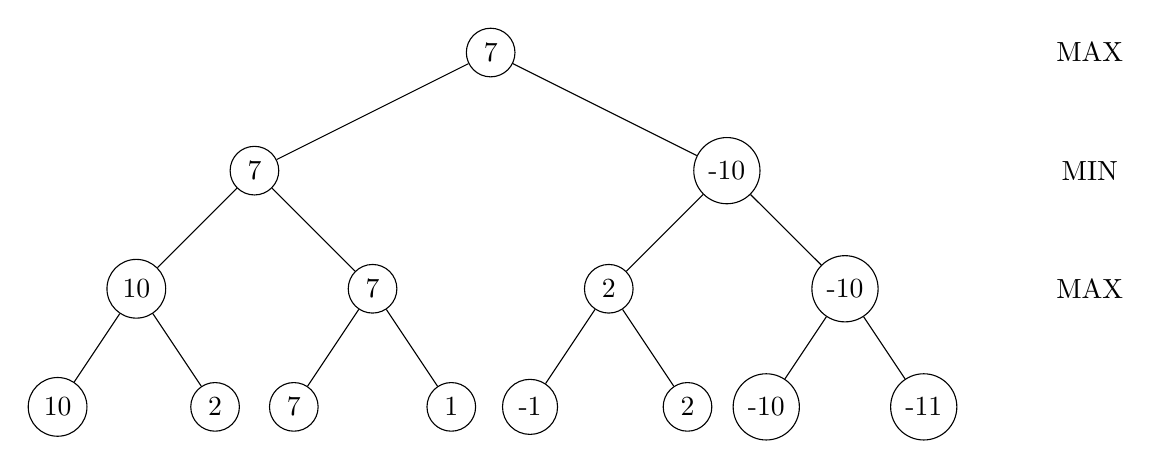
\begin{tikzpicture}[level/.style={sibling distance=60mm/#1}]
		\node [circle,draw] (z){7}
		  child {
		  	node [circle,draw] (a) {7}
		    child {
			    node [circle,draw] (b) {10}
			    child {
			    	node [circle,draw] {10}
			    } 
			    child {
			    	node [circle,draw] {2}
			    }
		    }
		    child {
		    	node [circle,draw] (g) {7}
		      	child {
		      		node [circle,draw] {7}
		   		}
		      	child {
		    		node [circle,draw] {1}
		   		}
		   	}
		  }
		  child {
		  	node [circle,draw] (j) {-10}
		    child {
		    	node [circle,draw] (k) {2}
		      	child {
		      		node [circle,draw] {-1}
		      	}
		      	child {
		      		node [circle,draw] {2}
		      	}
		    }
		  child {
		  	node [circle,draw] (l) {-10}
		    child {
		    	node [circle,draw] {-10}
		    }
		    child {
		    	node [circle,draw] {-11}
		    	child [grow=up] {
		    		node (s) {\hspace{10pc}MAX} edge from parent[draw=none]
		    		child [grow=up] {
		    			node (t) {\hspace{10pc}MIN} edge from parent[draw=none]
		    			child [grow=up] {
		    				node (u) {\hspace{10pc}MAX} edge from parent[draw=none]
		    			}
                	}
              	}
            }
		    }
		  };
		\end{tikzpicture}
		\vspace{1pc}
		\\
		The tree shown above contains all the values in the corresponding nodes in accordance to Minimax algorithm.
	\subsection{$\alpha$-$\beta$ Pruning}
		Alpha-Beta Pruning Tree\vspace{0.5pc}\\
		
		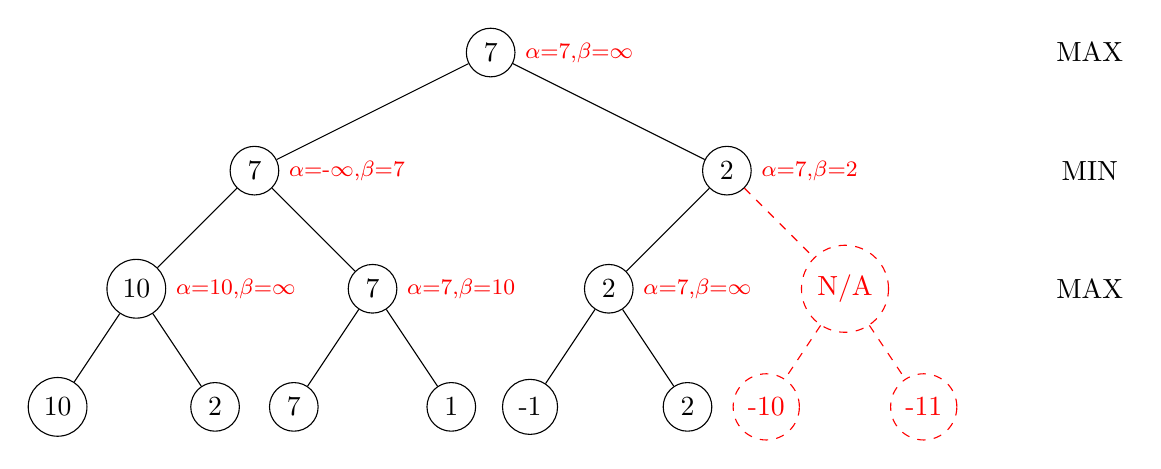
\begin{tikzpicture}[level/.style={sibling distance=60mm/#1}]
		\node [circle,draw,label=right:\textcolor{red}{\footnotesize$\alpha$=7,$\beta$=$\infty$}] (z){7}
		  child {
		  	node [circle,draw,label=right:\textcolor{red}{\footnotesize$\alpha$=-$\infty$,$\beta$=7}] (a) {7}
		    child {
			    node [circle,draw,label=right:\textcolor{red}{\footnotesize$\alpha$=10,$\beta$=$\infty$}] (b) {10}
			    child {
			    	node [circle,draw] {10}
			    } 
			    child {
			    	node [circle,draw] {2}
			    }
		    }
		    child {
		    	node [circle,draw,label=right:\textcolor{red}{\footnotesize$\alpha$=7,$\beta$=10}] (g) {7}
		      	child {
		      		node [circle,draw] {7}
		   		}
		      	child {
		    		node [circle,draw] {1}
		   		}
		   	}
		  }
		  child {
		  	node [circle,draw,label=right:\textcolor{red}{\footnotesize$\alpha$=7,$\beta$=2}] (j) {2}
		    child {
		    	node [circle,draw,label=right:\textcolor{red}{\footnotesize$\alpha$=7,$\beta$=$\infty$}] (k) {2}
		      	child {
		      		node [circle,draw] {-1}
		      	}
		      	child {
		      		node [circle,draw] {2}
		      	}
		    }
		  child[dashed] {
		  	node [circle,draw,red] (l) {N/A} edge from parent[red]
		    child[dashed] {
		    	node [circle,draw,red] {-10}
		    }
		    child[dashed] {
		    	node [circle,draw,red] {-11}
		    	child [grow=up] {
		    		node[black] (s) {\hspace{10pc}MAX} edge from parent[draw=none]
		    		child [grow=up] {
		    			node[black] (t) {\hspace{10pc}MIN} edge from parent[draw=none]
		    			child [grow=up] {
		    				node[black] (u) {\hspace{10pc}MAX} edge from parent[draw=none]
		    			}
                	}
              	}
            }
		    }
		  };
		\end{tikzpicture}
		\\
		\textbf{Note:} The pruned branches are shown in red dotted lines and curves.\\
	\subsection{Use of $\alpha$-$\beta$ Pruning}
		We use $\alpha$-$\beta$ Pruning in order to prevent the algorithm from traversing unnecessary branches of the search tree. This helps us to not waste time and use the time to perform a deeper search at the same time (reduce the effective depth of the search tree).
\end{document}

% Part c:
% Genetic algorithms undergo corssover wheras standard hillclimbing algorithms don't. This means that GA can get out of local maximas whereas hillclimbing can not. 

% Question 3:
% Part c:
% The benefit of alpha–beta pruning lies in the fact that branches of the search tree can be eliminated. This way, the search time can be limited to the 'more promising' subtree, and a deeper search can be performed in the same time
% The optimization reduces the effective depth to slightly more than half that of simple minimax if the nodes are evaluated in an optimal or near optimal order (best choice for side on move ordered first at each node)
